% Copyright (c) 2015 Daniele Masini - d.masini.it@gmail.com
% Copyright (c) 2016 Daniele Zambelli - daniele.zambelli@gmail.com

\begin{comment}

\begin{esercizio}
\label{ese:}
~

\noindent\begin{minipage}{.45\textwidth}

\end{minipage} 
\begin{minipage}{.55\textwidth}
\begin{inaccessibleblock}[Figura: TODO]
\begin{center} \input{\folder } \end{center}
\end{inaccessibleblock}
\end{minipage}
\end{esercizio}

\end{comment}

\section{Esercizi}

% \subsection{Esercizi riepilogativi - senza l'applicazione del sistema di 
% riferimento cartesiano}

\subsection{Trasformazioni nella geometria sintetica}

\begin{inaccessibleblock}[Figura: TODO]
 \begin{figure}[!htb]
  \centering% Copyright (c) 2015 Daniele Masini - d.masini.it@gmail.com

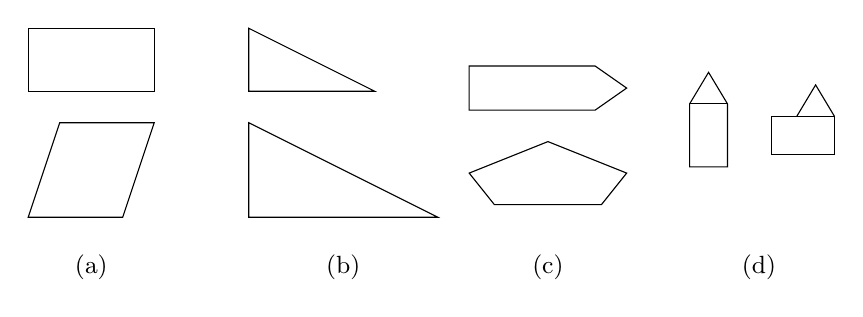
\begin{tikzpicture}[scale=0.8,font=\small]
\usetikzlibrary{calc}

\begin{scope}
\draw (0,0) rectangle (2,1);
\draw (0,-2) -- (1.5,-2) -- (2,-0.5) -- (0.5,-0.5) -- cycle;
\node at (1,-2.8) {(a)};
\end{scope}

\begin{scope}[xshift=3.5cm]
\draw (0,0) -- (0,1) -- (2,0) -- cycle;
\draw (0,-2) -- (0,-0.5) -- (3,-2) -- cycle;
\node at (1.5,-2.8) {(b)};
\end{scope}

\begin{scope}[xshift=7cm]
\begin{scope}[yshift=-0.3cm]
\draw (0,0) -- (0,0.7) -- (2,0.7) -- (2.5,0.35) -- (2,0) -- cycle;
\draw (0,-1) -- (1.25,-0.5) -- (2.5,-1) -- (2.1,-1.5) -- (0.4,-1.5) -- cycle;
\end{scope}
\node at (1.25,-2.8) {(c)};
\end{scope}

\begin{scope}[xshift=10.5cm]
\begin{scope}[yshift=-1.2cm]
\draw (0,0) -- (0,1) -- (0.3,1.5) -- (0.6,1) -- (0.6,0) -- cycle;
\draw (0,1) -- (0.6,1);
\end{scope}
\begin{scope}[xshift=1.3cm, yshift=-1cm]
\draw (0,0) -- (0,0.6) -- (1,0.6) -- (1,0) -- cycle;
\draw (0.4,0.6) -- (0.7,1.1) -- (1,0.6);
\end{scope}
\node at (1.1,-2.8) {(d)};
\end{scope}

\end{tikzpicture}

  \caption{Esercizio~\ref{ese:8.1}}\label{fig:ese8.1}
\end{figure}
\end{inaccessibleblock}

\begin{esercizio}
\label{ese:8.2}
Si sa che una trasformazione geometrica muta un quadrato in un rombo; 
gli invarianti di questa trasformazione sono:
\begin{enumeratea}
\item il parallelismo dei lati e l'ampiezza degli angoli;
\item l'ampiezza degli angoli e la misura dei lati;
\item solo il parallelismo   dei lati;
\item il parallelismo dei lati e la perpendicolarità delle diagonali.
\end{enumeratea}
\hfill [d]
\end{esercizio}

\begin{esercizio}
\label{ese:8.3}
Quali coppie rappresentate nella figura~\ref{fig:ese8.3} sono formate 
da figure corrispondenti in una isometria? \hfill [b, e]
\end{esercizio}


\begin{inaccessibleblock}[Figura: TODO]
 \begin{figure}[!htb]
  \centering% Copyright (c) 2015 Daniele Masini - d.masini.it@gmail.com

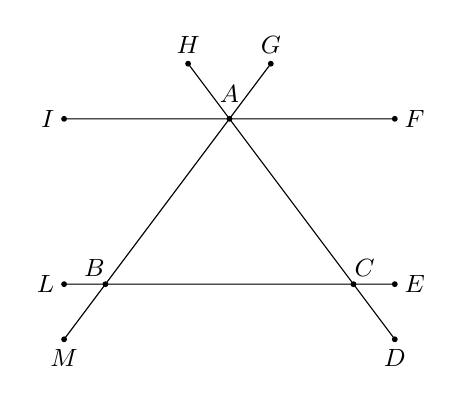
\begin{tikzpicture}[scale=0.7,font=\small, extended line/.style={shorten >=-#1,shorten <=-#1}, extended line/.default=1cm]
\usetikzlibrary{calc, through, intersections}

\begin{scope}
\coordinate (L) at (-3,-3);
\coordinate (E) at (3,-3);
\coordinate (I) at (-3,0);
\coordinate (F) at (3,0);
\coordinate (H) at (-0.75,1);
\coordinate (D) at (3,-4);
\coordinate (G) at (0.75,1);
\coordinate (M) at (-3,-4);

\coordinate (A) at (intersection of H--D and G--M);
\coordinate (B) at (intersection of L--E and G--M);
\coordinate (C) at (intersection of L--E and H--D);

\draw[fill] (I) circle (1.2pt) node[left] {$I$} -- (F) circle (1.2pt) node[right] {$F$};
\draw[fill] (L) circle (1.2pt) node[left] {$L$} -- (E) circle (1.2pt) node[right] {$E$};
\draw[fill] (H) circle (1.2pt) node[above] {$H$} -- (D) circle (1.2pt) node[below] {$D$};
\draw[fill] (G) circle (1.2pt) node[above] {$G$} -- (M) circle (1.2pt) node[below] {$M$};
\draw[fill] (A) circle (1.2pt) node[shift={(0pt,9pt)}] {$A$};
\draw[fill] (B) circle (1.2pt) node[shift={(-4pt,6pt)}] {$B$};
\draw[fill] (C) circle (1.2pt) node[shift={(4pt,6pt)}] {$C$};

\end{scope}

\end{tikzpicture}

  \caption{Esercizio~\ref{ese:8.3}}\label{fig:ese8.3}
\end{figure}
\end{inaccessibleblock}

\begin{esercizio}
\label{ese:8.4}
Presi nel piano due punti $T$ e $T'$ è vero che possiamo sempre 
individuare la simmetria centrale in cui $T'$ è immagine di $T$?
\end{esercizio}

\begin{esercizio}
\label{ese:8.5}
Come dobbiamo scegliere due segmenti affinché sia possibile 
determinare una simmetria centrale in cui essi siano corrispondenti?
\end{esercizio}

\begin{esercizio}
\label{ese:8.16}
Nel piano sono assegnati i punti $T$ e $T'$ corrispondenti in una 
simmetria assiale. Come potete determinare l'asse di simmetria?
\hfill[Falso]
\end{esercizio}

\noindent\begin{minipage}{0.6\textwidth}\parindent15pt
\begin{esercizio}
\label{ese:8.17}
Nel piano è assegnata la retta $r$ e un suo punto $P$ e un punto $P'$ 
non appartenente ad $r$. Costruisci la retta $r'$ immagine di $r$ 
nella simmetria assiale che fa corrispondere al punto $P$ il punto 
$P'$.
\end{esercizio}
\end{minipage}\hfil
\begin{minipage}{0.4\textwidth}
  \centering% Copyright (c) 2015 Daniele Masini - d.masini.it@gmail.com

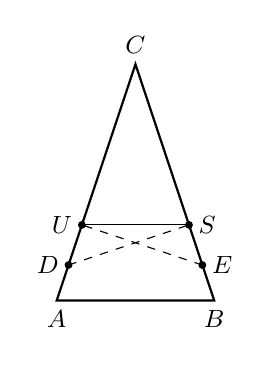
\begin{tikzpicture}[scale=1,font=\small, extended line/.style={shorten >=-#1,shorten <=-#1}, extended line/.default=1cm]
\usetikzlibrary{calc, through, intersections}

\begin{scope}
\coordinate (C) at (0,0);
\coordinate (A) at (-1,-3);
\coordinate (B) at (1,-3);
\coordinate (D) at ($(A)!0.15!(C)$);
\coordinate (E) at ($(B)!0.15!(C)$);
\coordinate (U) at ($(A)!(E)!(C)$);
\coordinate (S) at ($(B)!(D)!(C)$);

\draw[fill] (E) circle (1.2pt) node[right] {$E$};
\draw[fill] (D) circle (1.2pt) node[left] {$D$};
\draw[dashed] (E) -- (U);
\draw[fill] (U) circle (1.2pt) node[left] {$U$};
\draw[dashed] (D) -- (S);
\draw[fill] (S) circle (1.2pt) node[right] {$S$};
\draw (U) -- (S);

\draw[thick] (A) node[below] {$A$} -- (B) node[below] {$B$} -- (C) node[above] {$C$} -- cycle;

\end{scope}

\end{tikzpicture}

\end{minipage}\vspace{5pt}

\begin{esercizio}
\label{ese:8.18}
Costruite l'immagine di ciascun triangolo $ABC$ della 
figura~\ref{fig:ese8.18} nella simmetria avente come asse la retta 
del lato $AC$.
\end{esercizio}


\begin{inaccessibleblock}[Figura: TODO]
 \begin{figure}[!htb]
  \centering% Copyright (c) 2015 Daniele Masini - d.masini.it@gmail.com

\begin{tikzpicture}[scale=1.2,font=\small]
\usetikzlibrary{calc}

\begin{scope}
\draw (0,0) node[below left] {$A$} -- (0,2) node[above left] {$C$} -- (1.6,0.6) node[right] {$B$} -- cycle;
\node at (0.6,0.8) {$T_1$};
\end{scope}

\begin{scope}[xshift=3.2cm]
\draw (0,0) node[left] {$A$} -- (0,1.7) node[above left] {$B$} -- (2.3,0) node[right] {$C$} -- cycle;
\node at (0.7,0.6) {$T_2$};
\end{scope}

\begin{scope}[xshift=7cm]
\draw (0,0) node[left] {$A$} -- (1.5,0.7) node[above] {$C$} -- (3,0) node[right] {$B$} -- cycle;
\node at (1.5,0.3) {$T_3$};
\end{scope}

\end{tikzpicture}

  \caption{Esercizio~\ref{ese:8.18}}\label{fig:ese8.18}
\end{figure}
\end{inaccessibleblock}

\begin{esercizio}
\label{ese:8.19}
Nel triangolo isoscele $ABC$ di base $BC$ considerate la retta $r$ 
passante per $A$ e perpendicolare a $BC$; costruite l'immagine di 
$ABC$ nella simmetria di asse $r$. Stabilite quale proposizione è 
vera:
\begin{enumeratea}
\item il triangolo è fisso nella simmetria considerata;
\item il triangolo è unito nella simmetria considerata.
\end{enumeratea}
\end{esercizio}

\begin{esercizio}
\label{ese:8.20}
Assegnato il quadrato $ABCD$, determinate la sua immagine nella 
simmetria avente come asse la retta della diagonale $AC$. Stabilite 
quale proposizione è vera:
\begin{enumeratea}
\item il quadrato è fisso nella simmetria considerata;
\item il quadrato è unito nella simmetria considerata.
\end{enumeratea}
\end{esercizio}

\begin{esercizio}
\label{ese:8.21}
Motivate la verità delle proposizioni\\
$p_1$: <<il quadrato possiede 4 assi di simmetria>>,\\
$p_2$: <<il triangolo equilatero possiede 3 assi di simmetria>>.
\end{esercizio}

\begin{esercizio}
\label{ese:8.22}
Dimostrate che la retta di un diametro è asse di simmetria per la 
circonferenza. Potete concludere che la circonferenza possiede 
infiniti assi di simmetria?
\end{esercizio}

\begin{esercizio}
\label{ese:8.23}
Tra i trapezi ne trovate uno avente un asse di simmetria? Qual è 
l'asse di simmetria? 
\end{esercizio}

\noindent\begin{minipage}{0.8\textwidth}\parindent15pt
\begin{esercizio}
\label{ese:8.24}
Quali lettere dell'alfabeto, tra quelle proposte a fianco, hanno un 
asse di simmetria?
\end{esercizio}
\end{minipage}\hfil
\begin{minipage}{0.2\textwidth}
  \centering~~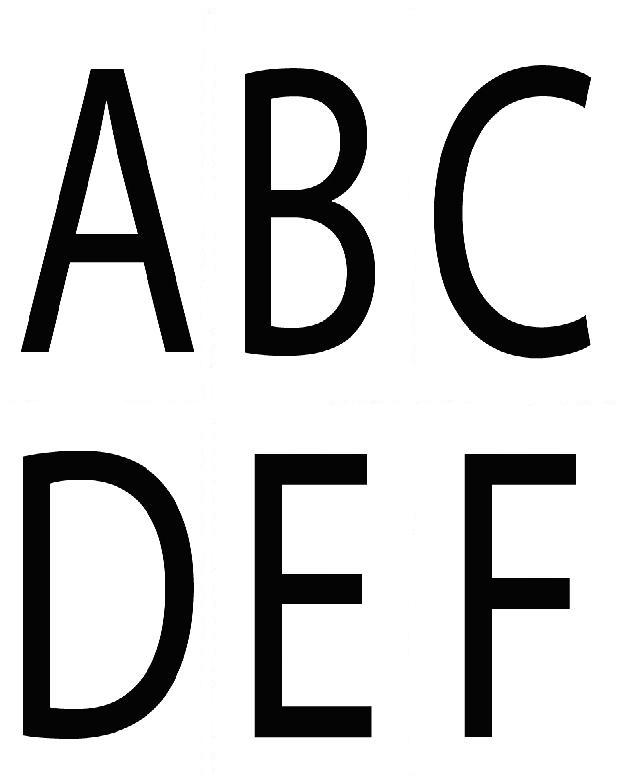
\includegraphics[width=0.7\textwidth]
  {\folder img/abcdef.png}
\end{minipage}\vspace{3pt}

\noindent\begin{minipage}{0.75\textwidth}\parindent15pt
\begin{esercizio}
  \label{ese:8.25}
  Le due rette tracciate sono assi di simmetria del rettangolo 
in grigio a fianco e pertanto lo sono anche per l'immagine in esso 
contenuta. Vero o falso?
\end{esercizio}
\end{minipage}\hfil
\begin{minipage}{0.25\textwidth}
  
\centering 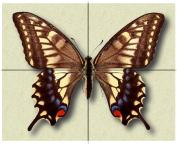
\includegraphics[width=0.75\textwidth]{\folder img/butterfly.png}
\end{minipage}%\vspace{5pt}

\begin{esercizio}
\label{ese:8.26}
Perché la retta che congiunge i punti medi dei lati obliqui di un 
trapezio isoscele non è un suo asse di simmetria?
\end{esercizio}

\newpage %---------------------------------------------------

\begin{esercizio}
\label{ese:8.40} % 47
Quale tra le seguenti caratteristiche è invariante in una simmetria 
assiale?
\begin{enumeratea}
\item la posizione della figura;
\item la direzione della retta;
\item il parallelismo;
\item l'orientamento dei punti;
\item dipende dall'asse di simmetria.
\end{enumeratea}
\end{esercizio}

\begin{esercizio}
\label{ese:8.41} % 48
I segmenti $AB$ e $A'B'$ si corrispondono nella simmetria di asse 
$r$; sapendo che $ABB'A'$ è un rettangolo, quale proposizione è vera?
\begin{enumeratea}
\item $AB$ è perpendicolare ad $r$;
\item $AB$ è parallelo ad $r$;
\item $AB$ appartiene ad $r$;
\item $AB$ è obliquo rispetto ad $r$ e $AB\cap r=H$.
\end{enumeratea}
\end{esercizio}

\begin{esercizio}
\label{ese:}
~

\noindent\begin{minipage}{.70\textwidth}
Nel piano sono assegnati i tre punti $A$, $B$ e $A'$ dei quali il 
punto $A'$ è immagine di $A$ in una traslazione. Dopo aver 
determinato il vettore della traslazione costruite l'immagine del 
triangolo $ABA'$.
\end{minipage} 
\begin{minipage}{.25\textwidth}
\begin{inaccessibleblock}[Figura: TODO]
\begin{center} % Copyright (c) 2015 Daniele Masini - d.masini.it@gmail.com

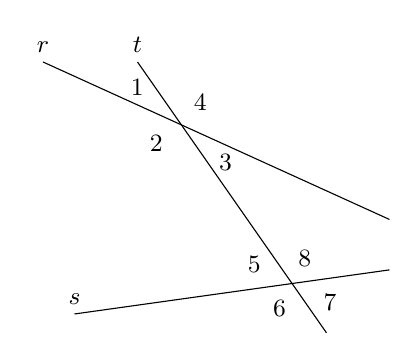
\begin{tikzpicture}[scale=0.8,font=\small, extended line/.style={shorten >=-#1,shorten <=-#1}, extended line/.default=1cm]
\usetikzlibrary{calc, through, intersections}

\begin{scope}
\coordinate (s1) at (0,0);
\coordinate (s2) at (5,0.7);
\coordinate (r1) at (-0.5,4);
\coordinate (r2) at (5,1.5);
\coordinate (t1) at (4,-0.3);
\coordinate (t2) at (1,4);

\coordinate (p1) at (intersection of s1--s2 and t1--t2);
\coordinate (p2) at (intersection of r1--r2 and t1--t2);

\node[black] at ([shift={(-0.7,0.6)}]p2) {$1$};
\node[black] at ([shift={(0.3,0.35)}]p2) {$4$};
\node[black] at ([shift={(-0.4,-0.3)}]p2) {$2$};
\node[black] at ([shift={(0.7,-0.6)}]p2) {$3$};

\node[black] at ([shift={(-0.6,0.3)}]p1) {$5$};
\node[black] at ([shift={(0.2,0.4)}]p1) {$8$};
\node[black] at ([shift={(-0.2,-0.4)}]p1) {$6$};
\node[black] at ([shift={(0.6,-0.3)}]p1) {$7$};

\draw (r1) node[above] {$r$} -- (r2);
\draw (s1) node[above] {$s$} -- (s2);
\draw (t1) -- (t2) node[above] {$t$};

\end{scope}

\end{tikzpicture}
 \end{center}
\end{inaccessibleblock}
\end{minipage}
\end{esercizio}

\begin{esercizio}
\label{ese:8.45} % 52
Determinate l'immagine del parallelogrammo $ABCD$ nella traslazione 
di vettore $\vec{v} \equiv \overrightarrow{AC}$.
\end{esercizio}

\begin{esercizio}
\label{ese:}
~

\noindent\begin{minipage}{.70\textwidth}
Dati due punti distinti $A$ e $B$ e il vettore $\overrightarrow{CD}$ 
della figura a fianco, detti $A'$ e $B'$ i punti immagine di $A$ e 
$B$ nella traslazione di vettore $\overrightarrow{CD}$, rispondete 
alle domande:
\begin{enumeratea}
\item Di che natura è il quadrilatero $ABB'A'$?
\item Può succedere che il quadrilatero in questione sia un 
rettangolo? E un rombo?
\item Cosa succede se $AB$ è parallelo al vettore 
$\overrightarrow{CD}$?
\end{enumeratea}
\end{minipage} 
\begin{minipage}{.28\textwidth}
\begin{inaccessibleblock}[Figura: TODO]
\begin{center} % Copyright (c) 2015 Daniele Masini - d.masini.it@gmail.com

\begin{tikzpicture}[scale=1,font=\small]
\usetikzlibrary{calc}

\begin{scope}
\draw[fill] (0,0) coordinate (c) circle (1pt) node[above right] {$C$};
\draw[fill] (1.7,0) coordinate (d) circle (1pt) node[above right] {$D$};
\draw[thick, blue, ->] (c) -- (d);
\draw[fill] (-0.4,-0.8) coordinate (a) circle (1pt) node[above right] {$A$};
\draw[fill] (0.7,-1.7) coordinate (b) circle (1pt) node[above right] {$B$};
\end{scope}

\end{tikzpicture}
 \end{center}
\end{inaccessibleblock}
\end{minipage}
\end{esercizio}

\begin{esercizio}
\label{ese:8.47} % 54
Come dobbiamo assegnare due segmenti $AB$ e $A'B'$ affinché siano 
corrispondenti in una traslazione? \`E unica la traslazione che 
associa ad $AB$ il segmento $A'B'$?
\end{esercizio}

\begin{esercizio}
\label{ese:}
~

\noindent\begin{minipage}{.70\textwidth}
Prendete in considerazione l'angolo $\epsilon$ di vertice $T$ della 
figura a fianco. Sia $O$ il centro di rotazione e $F$ un punto del 
piano di cui si vuole determinare l'immagine. Costruite $F'$ seguendo 
i passi illustrati immediatamente dopo la definizione~\ref{def:rotaz} 
a pagina~\pageref{def:rotaz}.
\end{minipage} 
\begin{minipage}{.28\textwidth}
\begin{inaccessibleblock}[Figura: TODO]
\begin{center} % Copyright (c) 2015 Daniele Masini - d.masini.it@gmail.com

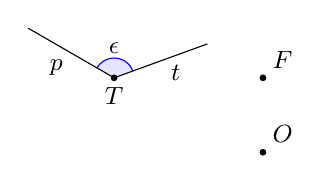
\begin{tikzpicture}[scale=1,font=\small, x=6.3mm, y=6.3mm, smooth]
\usetikzlibrary{calc}

\begin{scope}
\coordinate (t) at (0,0);
\coordinate (f) at (3,0);
\coordinate (o) at (3,-1.5);
\path (t) -- +(20:2) coordinate (t1);
\path (t) -- +(150:2) coordinate (t2);

\begin{scope}
\clip (t1) -- (t) -- (t2) -- cycle;
\draw[blue, fill=blue!10] (t) circle (0.4) node [black, shift={(90:0.6)}] {$\epsilon$};
\end{scope}

\draw (t) -- node[shift={(0.3,-0.25)}] {$t$} (t1);
\draw (t) -- node[shift={(-0.3,-0.3)}] {$p$} (t2);

\draw[fill] (t) circle (1pt) node [below] {$T$};
\draw[fill] (f) circle (1pt) node [above right] {$F$};
\draw[fill] (o) circle (1pt) node [above right] {$O$};

\end{scope}


\end{tikzpicture}
 \end{center}
\end{inaccessibleblock}
\end{minipage}
\end{esercizio}

\begin{esercizio}
\label{ese:8.59} % 69
Costruite l'immagine del quadrato $ABCD$ nella rotazione di 
$+90\grado$ avente come centro di simmetria il vertice $B$.
Fissate i punti medi $M$ ed $N$ rispettivamente di $AB$ e di $CD$; 
dove si trovano le rispettive immagini?
\end{esercizio}

\begin{esercizio}
\label{ese:8.62} % 72
Costruite l'immagine $A'B'C'$ del triangolo equilatero $ABC$ nella 
rotazione di centro $B$ e ampiezza $-120\grado$. Dimostrate che $C$, 
$B$ ed $A'$ sono allineati e che $ABC'$ è un triangolo equilatero 
congruente a quello dato.
\end{esercizio}

\begin{esercizio}
\label{ese:8.68} % 81
Giustificate la verità della proposizione: <<La simmetria centrale di 
centro $K$ è una rotazione di $180\grado$>>.
\end{esercizio}

\begin{esercizio}
\label{ese:}
~

\noindent\begin{minipage}{.70\textwidth}
Determinate l'immagine del punto $A$ nell'isometria $\Delta=S_b \circ 
S_a$ essendo $a$ e $b$ le rette parallele segnate nella figura a 
fianco e $A$ il punto dato. Dimostrate che $\overline{AA''}=2\cdot d$ 
essendo $d$ la distanza tra le rette $a$ e $b$.
Fissate arbitrariamente un altro punto $B$ non appartenente ad alcuna 
delle rette date e determinate la sua immagine $B''$ nell'isometria 
$\Delta$.
\`E vero che $\overline{AA''}=\overline{BB''}$ e $\overline{AA''} 
\parallel \overline{BB''}$? Potete concludere che l'isometria 
$\Delta$ è la traslazione di vettore $\overrightarrow{AA''}$?
\end{minipage} 
\begin{minipage}{.28\textwidth}
\begin{inaccessibleblock}[Figura: TODO]
\begin{center} % Copyright (c) 2015 Daniele Masini - d.masini.it@gmail.com

\begin{tikzpicture}[scale=1,font=\small]
\usetikzlibrary{calc}

\begin{scope}
\coordinate (a) at (0,0);

\draw[blue, thick] (-1.5,-0.5) -- (1.5,-0.5) node [black, above] {$a$};
\draw[blue, thick] (-1.5,-1.5) -- (1.5,-1.5) node [black, above] {$b$};

\draw[fill] (a) circle (1pt) node [above right] {$A$};

\end{scope}


\end{tikzpicture}

 \end{center}
\end{inaccessibleblock}
\end{minipage}
\end{esercizio}

% \begin{esercizio}
% \label{ese:8.74} % 87
% \noindent\begin{minipage}{0.75\textwidth}\parindent15pt
% 
% \end{minipage}\hfil
% \begin{minipage}{0.3\textwidth}
%   \centering~~\input{\folder }
% \end{minipage}\vspace{8pt}
% \end{esercizio}

\begin{esercizio}
\label{ese:8.75} % 88
Facendo riferimento all'esercizio~\ref{ese:8.74}, verificate che la 
traslazione $\Delta_1 = S_a \circ S_b$ è caratterizzata da un vettore 
avente modulo e direzione uguali al vettore $\overrightarrow{AA''}$ 
ma verso opposto.
\end{esercizio}

\begin{esercizio}
\label{ese:8.82} % 96
Verificate che:
\begin{enumeratea}
\item l'inversa della traslazione di vettore $\vec{v}(a;b)$ è la 
traslazione di vettore $-\vec{v}$;
\item l'inversa di una rotazione di centro $O$ e angolo $\alpha$ è la 
rotazione di centro $O$ e angolo $-\alpha$.
\end{enumeratea}
\end{esercizio}

\begin{esercizio}
\label{ese:8.83} % 97
Verificate che le simmetrie (centrale e assiale) hanno se stesse come 
isometria inversa, ossia $(S_K)^{-1}=S_K$ e $(S_r)^{-1}=S_r$.
\end{esercizio}

\begin{esercizio}
\label{ese:8.84} % 98
La proposizione <<la simmetria centrale è la composizione di due 
simmetrie assiali>> è:
\begin{enumeratea}
\item sempre vera;
\item vera se i due assi sono incidenti;
\item mai vera;
\item vera se i due assi sono perpendicolari;
\item vera se i due assi sono paralleli.
\end{enumeratea}
\end{esercizio}

\begin{esercizio}
\label{ese:8.86} % 100
Stabilite il valore di verità delle proposizioni:
%Componendo due isometrie si ottiene una isometria
\begin{enumeratea}
\item Componendo due simmetrie assiali si ottiene una simmetria 
assiale\hfill\boxV\quad\boxF
\item Componendo due traslazioni si ottiene una 
traslazione\hfill\boxV\quad\boxF
\item Componendo due simmetrie centrali si ottiene una simmetria 
centrale\hfill\boxV\quad\boxF
\item Componendo due simmetrie assiali di assi incidenti si ottiene 
una rotazione\hfill\boxV\quad\boxF
\item Componendo due rotazioni si ottiene una 
rotazione\hfill\boxV\quad\boxF
\item L'identità si ottiene componendo una isometria con sé 
stessa\hfill\boxV\quad\boxF
\item L'inversa di una traslazione è la stessa 
traslazione\hfill\boxV\quad\boxF
\item Componendo una simmetria centrale con una rotazione si ottiene 
l'identità\hfill\boxV\quad\boxF
\item Componendo una simmetria centrale di centro $H$ con la 
simmetria assiale avente \\
come asse una retta passante per $H$ si ottiene sempre l'identità
\hfill\boxV\quad\boxF
\end{enumeratea}
\end{esercizio}


\begin{esercizio}
\label{ese:8.90} % 104
Attribuisci il valore di verità alle seguenti proposizioni:
\begin{enumeratea}
\item In una isometria vi è almeno un elemento 
unito\hfill\boxV\quad\boxF
\item Nella simmetria centrale vi sono infinite rette unite, ma 
solamente \\
un punto unito\hfill\boxV\quad\boxF
\item In ogni triangolo vi è almeno un asse di 
simmetria\hfill\boxV\quad\boxF
\item Qualche quadrilatero ha un centro di 
simmetria\hfill\boxV\quad\boxF
\item Il triangolo equilatero ha un centro di 
simmetria\hfill\boxV\quad\boxF
\item Il rombo è l'unico quadrilatero avente due assi di 
simmetria\hfill\boxV\quad\boxF
\item Tutte le rette aventi la stessa direzione del vettore della 
traslazione sono unite\hfill\boxV\quad\boxF
\item Solo la simmetria assiale è una isometria 
invertente\hfill\boxV\quad\boxF
\item Rette parallele hanno come immagine in una isometria rette 
parallele\hfill\boxV\quad\boxF
\item In una isometria una retta è sempre parallela alla sua 
immagine\hfill\boxV\quad\boxF
\end{enumeratea}
\end{esercizio}


\begin{esercizio}
\label{ese:}
~

\noindent\begin{minipage}{.70\textwidth}
I due segmenti della figura a fianco possono essere corrispondenti in 
una simmetria centrale?
\end{minipage} 
\begin{minipage}{.28\textwidth}
\begin{inaccessibleblock}[Figura: TODO]
\begin{center} % Copyright (c) 2015 Daniele Masini - d.masini.it@gmail.com

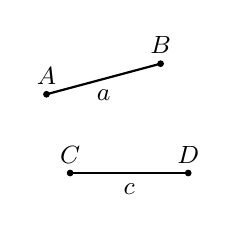
\begin{tikzpicture}[scale=1,font=\small]
\usetikzlibrary{calc}

\begin{scope}
\coordinate (a) at (0,0);
\path (a) -- +(15:1.5) coordinate (b);
\coordinate (c) at (0.3,-1);
\path (c) -- +(0:1.5) coordinate (d);

\draw[thick] (a) -- node [below] {$a$} (b);
\draw[thick] (c) -- node [below] {$c$} (d);

\draw[fill] (a) circle (1pt) node [above] {$A$};
\draw[fill] (b) circle (1pt) node [above] {$B$};
\draw[fill] (c) circle (1pt) node [above] {$C$};
\draw[fill] (d) circle (1pt) node [above] {$D$};

\end{scope}


\end{tikzpicture}

 \end{center}
\end{inaccessibleblock}
\end{minipage}
\end{esercizio}

% \begin{esercizio}
% \label{ese:8.94} % 108
% \noindent\begin{minipage}{0.75\textwidth}\parindent15pt
% 
% \end{minipage}\hfil
% \begin{minipage}{0.25\textwidth}
%   \centering~~\input{\folder }
% \end{minipage}\vspace{8pt} 
% \end{esercizio}

\begin{esercizio}
\label{ese:8.96} % 110
Costruite l'immagine di un triangolo rettangolo $ABC$ (non isoscele) 
di ipotenusa $BC$
\begin{enumeratea}
\item in ciascuna delle simmetrie $S_A$, $S_B$ e $S_C$;
\item nella simmetria $S_M$ essendo $M$ il punto medio dell'ipotenusa;
\item in ciascuna delle simmetrie aventi come assi le rette dei lati.
\end{enumeratea}
\end{esercizio}

\begin{esercizio}
  \label{ese:8.63} % 73
  Nel piano è assegnato il punto $C$ e il vettore $\vec{v}$ (figura a 
  lato); costruite l'immagine del punto $P$ nell'isometria $T_{\vec{v}} 
  \circ S_{C}$ e anche l'immagine dello stesso punto $P$ nell'isometria 
  $S_{C} \circ T_{\vec{v}}$. Determinate l'equazione di $\Phi_1 = 
  T_{\vec{v}} \circ S_{C}$ e di $\Phi_2 = S_{C} \circ T_{\vec{v}}$.
\end{esercizio}

% \subsection{Esercizi riepilogativi - con l'applicazione del sistema di 
% riferimento cartesiano}

\subsection{Trasformazioni nella geometria analitica}

\begin{esercizio}
  \label{ese:8.7}
  Sappiamo che $S_K:P\left(\frac{3}{5};0\right) \rightarrow 
  P'\left(-\frac{2}{3};-\frac{1}{2}\right)$, determinate il centro $K$ 
  della simmetria. 
\end{esercizio}

\begin{esercizio}
  \label{ese:8.8}
  Il segmento di estremi $A(-2;4)$ e $B(2;-4)$ in $S_O$, essendo $O$ 
  l'origine del riferimento cartesiano ortogonale
  \begin{enumeratea}
    \item ha tutti i suoi punti fissi;
    \item ha un solo punto fisso;
    \item ha fissi solo gli estremi;
    \item ha fissi tutti i punti interni ma non gli estremi;
    \item non ha punti fissi.
  \end{enumeratea}
\end{esercizio}

\begin{esercizio}
  \label{ese:8.9}
  Sono assegnati i punti $A(-5;0)$, $B(0;5)$ e $C(1;-1)$; determinate 
  le coordinate dei vertici $A'B'C'$ del triangolo immagine di $ABC$ 
  nella simmetria avente come centro il punto medio $M$ del lato $AC$.
\end{esercizio}

\begin{esercizio}
  \label{ese:8.10}
  I punti $A(1;5)$, $B(-2;2)$ e $C(0;-4)$ sono tre vertici di un 
  parallelogramma. Determinate le coordinate del quarto vertice. 
  Indicate con $M$ il punto di incontro delle diagonali; in $S_M$ il 
  parallelogramma $ABCD$ è fisso o unito? Perché?
\end{esercizio}

\begin{esercizio}
  \label{ese:8.13}
  Il centro della simmetria che associa al triangolo di vertici 
  $A(0;4)$, $B(-2;1)$ e $C(1;5)$ il triangolo di vertici $A'(2;-2)$, 
  $B'(4;1)$ e $C'(1;-3)$ è
  \begin{multicols}{2}
    \begin{enumeratea}
      \item $K(-1;1)$;
      \item $K(1;-1)$;
      \item $K(1;1)$;
      \item $K(-1;-1)$.
    \end{enumeratea}
  \end{multicols}
\end{esercizio}

\begin{esercizio}
  \label{ese:8.14}
  Determinate l'immagine $M'$ del punto medio $M$ del segmento $AB$ di 
  estremi $A(0;5)$ e $B(-4;1)$ in $S_O$ ($O$ è l'origine del 
  riferimento cartesiano). \`E vero che $BM'A$ è isoscele sulla base 
  $AB$?
\end{esercizio}

\begin{esercizio}
  \label{ese:8.15}
  Determinate la natura del quadrilatero $ABA'B$ che si ottiene 
  congiungendo nell'ordine i punti $A(-1;1)$, $B(-4;-5)$, $A'$ e $B'$ 
  rispettivamente simmetrici di $A$ e $B$ in $S_O$. Determinate la 
  misura delle sue diagonali.
\end{esercizio}

\begin{esercizio}
  \label{ese:8.27}
  In $S_x$ (simmetria assiale rispetto all'asse $x$) il segmento $AB$ 
  di estremi $A(3;2)$ e $B(3;-2)$
  \begin{enumeratea}
    \item è unito, luogo di punti uniti;
    \item non ha punti fissi;
    \item ha tutti i suoi punti uniti tranne $A$ e $B$;
    \item ha un solo punto fisso;
    \item ha solo $A$ e $B$ fissi.
  \end{enumeratea}
\end{esercizio}

\begin{esercizio}
  \label{ese:8.29} % 33
  Il triangolo $ABC$ è isoscele; sapendo che $A(0;4)$, $B(-2;0)$ e che 
  l'asse $x$ è il suo asse di simmetria, determinate il vertice $C$, il 
  perimetro e l'area del triangolo.
\end{esercizio}

\begin{esercizio}
  \label{ese:8.30} % 34
  Il triangolo $ABC$ è isoscele; sapendo che $A(0;4)$, $B(-2;0)$ e che 
  l'asse $y$ è il suo asse di simmetria, determinate il vertice $C$, il 
  perimetro e l'area del triangolo.
\end{esercizio}

\begin{esercizio}
  \label{ese:8.34} % 41
  Nella simmetria $S_{b1}$ la retta $y=-x$ è fissa o unita?
\end{esercizio}

\begin{esercizio}
  \label{ese:8.35} % 42
  Motivate la verità della seguente proposizione: <<nella simmetria 
  $S_{b2}$ l'immagine dell'asse $x$ è l'asse $y$>>. Viene mantenuto 
  l'orientamento dell'asse $x$?
  Completate: $S_{b2}:(\text{asse }x)\rightarrow (\text{asse } 
  \ldots{})$ e $(\text{asse }y)\rightarrow(\ldots\ldots{})$
  Analogamente: $S_{b1}:(\text{asse }x)\rightarrow (\text{asse } 
  \ldots{})$ e $(\text{asse }y)\rightarrow(\ldots\ldots{})$
\end{esercizio}

\begin{esercizio}
  \label{ese:8.36} % 43
  Dato il quadrilatero $ABCD$ di vertici $A(0;0)$, $B(3;1)$, $C(4;4)$ e 
  $D(1;3)$ trovate il suo corrispondente in $S_{b1}$. Quale delle 
  seguenti affermazioni ritenete corretta:
  \begin{enumeratea}
    \item il quadrilatero è fisso nella simmetria considerata;
    \item il quadrilatero è unito nella simmetria considerata.
  \end{enumeratea}
\end{esercizio}

\begin{esercizio}
  \label{ese:8.38} % 45
  Nel piano cartesiano sono assegnati i punti $A(0;3)$, $B(-2;0)$ e 
  $C(-1;-3)$.
  \begin{enumeratea}
    \item Determinate i punti $A'$, $B'$ e $C'$ immagine in $S_{b2}$.
    \item Calcolate l'area del quadrilatero $A'B'C'O$, essendo $O$ 
    l'origine del riferimento.
    \item Motivate la verità della proposizione: <<i segmenti $AB$ e 
    $A'B'$ si incontrano in un punto $P$ della bisettrice del 
    II\textsuperscript{o}-IV\textsuperscript{o} quadrante>>.
    \item \`E vero che $AP'B$ è congruente a $PAB'$?
  \end{enumeratea}
\end{esercizio}

\begin{esercizio}
  \label{ese:8.39} % 46
  Sono assegnate le simmetrie
  \[S_1:\begin{cases}x'=-x\\y'=-y\end{cases};\quad 
  S_2:\begin{cases}x'=y\\y'=x\end{cases};\quad
  S_3:\begin{cases}x'=2-x\\y'=y\end{cases};\quad 
  S_4:\begin{cases}x'=-x-1\\y'=3-y\end{cases}\]
  Usando qualche punto scelto arbitrariamente riconosci ciascuna di 
  esse e completa la tabella sottostante:
  \begin{center}
    \begin{tabular}{cccc}
      \toprule
      Simmetria & Tipo & Centro (coordinate) & Asse (equazione)\\
      \midrule
      $S_1$ & \ldots\ldots\ldots{} & \ldots\ldots{} & \ldots\ldots\ldots{} 
      \\
      $S_2$ & \ldots\ldots\ldots{} & \ldots\ldots{} & \ldots\ldots\ldots{} 
      \\
      $S_3$ & \ldots\ldots\ldots{} & \ldots\ldots{} & \ldots\ldots\ldots{} 
      \\
      $S_4$ & \ldots\ldots\ldots{} & \ldots\ldots{} & \ldots\ldots\ldots{} 
      \\
      \bottomrule
    \end{tabular}
  \end{center}
\end{esercizio}

\begin{esercizio}
  \label{ese:8.43} % 50
  Un segmento unito in $S_{b2}$ è
  \begin{enumeratea}
    \item un segmento perpendicolare alla bisettrice del 
    I\textsuperscript{o}-III\textsuperscript{o} quadrante;
    \item un segmento perpendicolare alla bisettrice del 
    II\textsuperscript{o}-IV\textsuperscript{o} quadrante nel suo punto 
    medio;
    \item un segmento parallelo alla bisettrice del 
    I\textsuperscript{o}-III\textsuperscript{o} quadrante;
    \item un segmento perpendicolare alla bisettrice del 
    II\textsuperscript{o}-IV\textsuperscript{o} quadrante;
    \item un segmento avente il suo punto medio appartenente alla 
    bisettrice del II\textsuperscript{o}-IV\textsuperscript{o} quadrante.
  \end{enumeratea}
\end{esercizio}

\begin{esercizio}
  \label{ese:8.48} % 58
  Nel riferimento cartesiano è assegnato il punto $P(-4;2)$. 
  Determinate il punto $P'$ immagine nella traslazione 
  $T(3;-1):\begin{cases}x'=x+3\\y'=y+(-1)\end{cases}$.\\
  Strategia risolutiva:
  \begin{enumerate*}
    \item individuate il vettore $\vec{w}$ della traslazione: 
    $\vec{w}(\ldots{};\ldots{})$;
    \item tracciate il vettore nel riferimento cartesiano;
    \item determinate le coordinate di $P'$: $P'(\ldots{};\ldots{})$.
  \end{enumerate*}
  Completate: $\overrightarrow{PP'}$ è \ldots\ldots\ldots{} a 
  $\vec{w}$; questo significa che i due vettori hanno 
  \ldots\ldots\ldots{} direzione (cioè sono \ldots\ldots\ldots{}), 
  stesso \ldots\ldots\ldots{} e \ldots\ldots\ldots{} intensità.
\end{esercizio}


\begin{esercizio}
  \label{ese:8.51} % 61
  Dopo aver determinato l'equazione della traslazione in cui $A'(0;-2)$ 
  è l'immagine di $A(3;2)$, determinate il perimetro del triangolo 
  $AO'A'$ essendo $O'$ il corrispondente di $O(0;0)$ nella traslazione 
  trovata.
\end{esercizio}

\begin{esercizio}
  \label{ese:8.52} % 62
  Verificate che il punto medio $M$ del segmento $PQ$ di estremi 
  $P(-1;4)$ e $Q(5;0)$ ha come immagine in $T(3;-1)$ il punto medio 
  $M'$ del segmento $P'Q'$.
\end{esercizio}

\begin{esercizio}
  \label{ese:8.53} % 63
  Applica la traslazione di equazione 
  $\begin{cases}x'=x+2\\y'=y-1\end{cases}$ al segmento di estremi 
  $A(-2;4)$ e $B(3;3)$. 
\end{esercizio}

\begin{esercizio}
  \label{ese:8.55} % 65
  Determinate l'immagine del triangolo di vertici $A(0;2)$, $B(-3;2)$ e 
  $C(0;5)$ nella traslazione $T(4;1)$. Calcolatene quindi perimetro e 
  area.
\end{esercizio}

% \begin{esercizio}
%   \label{ese:8.56} % 66
%   Determinate l'equazione della traslazione di vettore 
%   $\vec{s}=\vec{u}+\vec{v}$ assegnati dalla figura~\ref{fig:ese8.56}. 
%   Determinate inoltre l'immagine del poligono di vertici $H(-1;1)$, 
%   $K(0;-2)$, $L(3;0)$ ed $F(1;2)$.
% \end{esercizio}
% 
% 
% \begin{minipage}{0.25\textwidth}
%   \centering~~% Copyright (c) 2015 Daniele Masini - d.masini.it@gmail.com

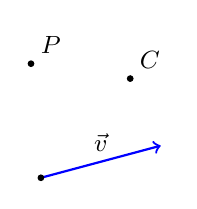
\begin{tikzpicture}[scale=1,font=\small, x=6.3mm, y=6.3mm, smooth]
\usetikzlibrary{calc}

\begin{scope}
\coordinate (v) at (0,0);
\coordinate (c) at (1.8,2);
\coordinate (p) at (-.2,2.3);
\path (v) -- +(15:2.5) coordinate (v1);

\draw[blue, thick, ->] (v) -- node [black, above] {$\vec{v}$} (v1);

\draw[fill] (v) circle (1pt);
\draw[fill] (c) circle (1pt) node [above right] {$C$};
\draw[fill] (p) circle (1pt) node [above right] {$P$};

\end{scope}


\end{tikzpicture}

% \end{minipage}\vspace{8pt}

\begin{esercizio}
  \label{ese:8.65} % 75
  Sono assegnati il punto $C(-4;3)$, la retta $x=1$ e il punto 
  $P(0;5)$. Determinate l'immagine $P''$ di $P$ nell'isometria 
  $\Delta=S_{C}\circ S_{x=1}$ e l'immagine $P^*$ di $P$ nell'isometria 
  $\Delta=S_{x=1}\circ S_{C}$. \`E vero che $P''$ e $P^*$ si 
  corrispondono nella simmetria $S_y$? Determinate l'area del triangolo 
  $PP''P^*$.
\end{esercizio}

\begin{esercizio}
  \label{ese:8.69} % 82
  Nel piano dotato di riferimento cartesiano è tracciata la bisettrice 
  del I e III quadrante e la 
  retta $y=1$. Completate le osservazioni seguenti:
  \begin{enumeratea}
    \item il punto di intersezione $K$ ha coordinate 
    $K(\ldots{};\ldots{})$;
    \item l'angolo delle due rette è di $\ldots{}\grado$.
  \end{enumeratea}
  Scrivete l'equazione della simmetria avente come asse la bisettrice: 
  $S_{b1}\begin{cases}x'=\ldots{}\\y'=\ldots{}\end{cases}$ e 
  l'equazione della simmetria di asse la retta $y=1$: 
  $S_{y=1}\begin{cases}x'=\ldots{}\\y'=\ldots{}\end{cases}$.

  Determinate le coordinate del punto $P''$ immagine di $P$, 
  arbitrariamente scelto, in $\Omega = S_{b1} \circ S_{y=1}$ e scrivete 
  l'equazione di $\Omega$.
  Concludete: $\Omega$ è la rotazione di centro \ldots{} e angolo 
  \ldots{} (ricordate il segno dell'angolo di rotazione).

  Determinate le coordinate del punto $P^*$ immagine di $P$, 
  arbitrariamente scelto, in $\Omega^*=S_{y=1} \circ S_{b1}$ e scrivete 
  l'equazione di $\Omega^*$.
  Concludete: $\Omega^*$ è la rotazione di centro \ldots{} e angolo 
  \ldots{} (ricordate il segno dell'angolo di rotazione).
\end{esercizio}

\begin{esercizio}
  \label{ese:8.73} % 86
  Determinate l'equazione della isometria $J=S_{b1} \circ S_{x=4}$ e 
  stabilite se esiste qualche elemento unito. Come cambia l'equazione 
  dell'isometria $J^*=S_{x=4} \circ S_{b1}$ rispetto alla precedente? 
  Sia $J$ che $J^*$ sono rotazioni: determinate centro e angolo (con 
  segno) di ognuna di esse. A questo scopo potete utilizzare il punto 
  $P(2;4)$ o un punto arbitrariamente scelto.
\end{esercizio}

\begin{esercizio}
  \label{ese:8.77} % 90
  Determinate i vettori $\vec{u}$ e $\vec{v}$ delle traslazioni 
  $T_{\vec{u}}\begin{cases}x'=x+1\\y'=y-2\end{cases}$ e 
  $T_{\vec{v}}\begin{cases}x'=x-3\\y'=y-1\end{cases}$ e il vettore 
  $\vec{s} = \vec{u} + \vec{v}$. Verificate che $T_{\vec{s}} = 
  T_{\vec{u}} \circ T_{\vec{v}}$.
  Cosa otteniamo dalla composizione $T_{\vec{u}} \circ T_{\vec{v}}$? 
  Sapresti darne la motivazione?
  Concludete: componendo due traslazioni si ottiene \ldots\ldots{}
\end{esercizio}

\begin{esercizio}
  \label{ese:8.78} % 91
  Nel riferimento cartesiano ortogonale $Oxy$ è assegnato il punto 
  $O_1(2;1)$; scrivete l'equazione della simmetria centrale di centro 
  $O$ $S_O\begin{cases}x'=\ldots{}\\y'=\ldots{}\end{cases}$  e 
  l'equazione della simmetria centrale di centro $O_1$ 
  $S_{O_1}\begin{cases}x'=\ldots{}\\y'=\ldots{}\end{cases}$. 
  Determinate l'immagine $P''$ del punto $P(1;2)$ nell'isometria 
  $\Sigma=S_O \circ S_{O_1}$ di cui avrete scritto l'equazione e 
  determinate $\overline{PP''}$. Determinate $Q''$ immagine di 
  $Q\left(\frac{1}{2};-1\right)$ nell'isometria $\Sigma$ e determinate 
  $\overline{QQ''}$. Potete affermare che $\overrightarrow{PP''} \equiv 
  \overrightarrow{QQ''}$? Verificate che $\overrightarrow{PP''} \equiv 
  \overrightarrow{QQ''} \equiv 2\cdot \overrightarrow{O_1O}$.
  \`E vero che $\Sigma=S_O \circ S_{O_1}$ e $\Sigma_1=S_{O_1} \circ 
  S_{O}$ sono la stessa isometria?
\end{esercizio}

\begin{esercizio}
  \label{ese:8.87} % 101
  L'equazione $\begin{cases}x'=4-x\\y'=y\end{cases}$ descrive: 
  \begin{enumeratea}
    \item la simmetria assiale di asse $y$;
    \item la simmetria assiale di asse la retta $x=4$;
    \item la traslazione di vettore $\vec{v}(4;0)$;
    \item la simmetria assiale di asse $x=2$;
    \item la simmetria centrale di centro $C(4;0)$.
  \end{enumeratea}
\end{esercizio}

\begin{esercizio}
  \label{ese:8.88} % 102
  La trasformazione $\Sigma \begin{cases}x'=-y+2\\y'=2x\end{cases}$ è 
  un'isometria?
\end{esercizio}

\begin{esercizio}
  \label{ese:8.89} % 103
  Il segmento di estremi $A(3;4)$ e $B(3;-2)$ ha come simmetrico il 
  segmento di estremi $A'(3;2)$ e $B'(5;2)$; è stata eseguita:
  \begin{enumeratea}
    \item la simmetria assiale di asse la retta $x=4$;
    \item la simmetria $S_{b2}$;
    \item la simmetria $S_{b1}$;
    \item la simmetria assiale di asse la retta $x=3$;
    \item la simmetria $S_{y=3}$.
  \end{enumeratea}
\end{esercizio}

\begin{esercizio}
  \label{ese:8.97} % 111
  Comporre due traslazioni di vettori $\vec{v_1}(2;3)$ e 
  $\vec{v_2}(3;6)$ applicandole al triangolo $ABC$ con $A(-2;-1)$, 
  $B(-1;-2)$ e $C(-4;-3)$.
\end{esercizio}

\begin{esercizio}
  \label{ese:8.98} % 112
  Determina il corrispondente $A'B'$ del segmento di vertici $A(-2;6)$ 
  e $B(-3;3)$ nella simmetria di asse $x=-1$. Applica poi al segmento 
  ottenuto un'ulteriore simmetria con asse $x=4$. Utilizzando 
  l'equazione per la composizione di due simmetrie con assi paralleli 
  tra loro, trova le nuove coordinate dei due punti $A$ e $B$.
\end{esercizio}

\begin{esercizio}
  \label{ese:8.99} % 113
  Determina il corrispondente $A'B'$ del segmento di vertici $A(1;-6)$ 
  e $B(4;3)$ nella simmetria di asse $x = 2$, applica poi al segmento 
  ottenuto un'ulteriore simmetria con asse $y = 1$. Utilizzando 
  l'equazione per la composizione di due simmetrie con assi 
  perpendicolari tra loro, determina le nuove coordinate dei due punti 
  $A$ e $B$.
\end{esercizio}

\begin{esercizio}
  \label{ese:8.101} % 115
  Sono assegnate le simmetrie assiali
  \[S_1 \begin{cases}x'=x\\y'=2-y\end{cases}\quad  S_2 
  \begin{cases}x'=-x\\y'=y\end{cases}\quad S_3 
  \begin{cases}x'=x\\y'=y\end{cases}\quad S_4 
  \begin{cases}x'=-x-6\\y'=y\end{cases}\]
  \begin{enumeratea}
    \item Individuate l'asse di simmetria di ciascuna di esse, 
    rappresentate nel riferimento cartesiano ortogonale i rispettivi assi 
    indicandoli con $s_1$, $s_2$, $s_3$ e $s_4$; completate e riproducete 
    nello stesso riferimento
    
    \begin{center}
      \begin{tabular}{cc}
        $P\left(-3;\frac{1}{2}\right)\overset{S_1}\longrightarrow 
        P_1(\ldots{};\ldots{})$ & 
        $P\left(-3;\frac{1}{2}\right)\overset{S_2}\longrightarrow 
        P_2(\ldots{};\ldots{})$\\
        $P\left(-3;\frac{1}{2}\right)\overset{S_3}\longrightarrow 
        P_3(\ldots{};\ldots{})$ & 
        $P\left(-3;\frac{1}{2}\right)\overset{S_4}\longrightarrow 
        P_4(\ldots{};\ldots{})$\\
      \end{tabular}
    \end{center}
    
    \item Siano $A$, $B$, $C$ e $D$ i punti $A=s_4\cap s_3$, $B=s_4\cap 
    s_1$, $C=s_1\cap s_3$ e $D=s_2\cap s_1$; dimostrate che i triangoli 
    $ABC$ e $CDE$ sono rettangoli isosceli e che i lati dell'uno sono il 
    quadruplo di quelli dell'altro.
    \item Determinate il rapporto tra i loro perimetri e tra le loro aree.
  \end{enumeratea}
\end{esercizio}

%\end{multicols}
